% テクニカルレポート（日本語版）。ビルド: bash docs/report/build.sh
\documentclass[10pt,a4paper,twocolumn]{article}
\usepackage[margin=17mm,columnsep=6mm]{geometry}
\usepackage{amsmath,amssymb}
\usepackage{booktabs}
\usepackage{graphicx}
\usepackage{xcolor}
\usepackage{tikz}
\usetikzlibrary{positioning,arrows.meta,fit,calc}
\usepackage[font=small,labelfont=bf,labelsep=quad]{caption}
\usepackage{enumitem}
\setlist{nosep,leftmargin=*}
\usepackage{xeCJK}
\setCJKmainfont[Path=fonts/,BoldFont=NotoSerifJP-Bold.otf]{NotoSerifJP-Regular.otf}
\setCJKsansfont[Path=fonts/,BoldFont=NotoSansJP-Bold.otf]{NotoSansJP-Regular.otf}
\usepackage[colorlinks=true,linkcolor=blue!50!black,citecolor=blue!50!black,urlcolor=blue!50!black]{hyperref}
\renewcommand{\abstractname}{概要}
\renewcommand{\refname}{参考文献}
\renewcommand{\figurename}{図}
\renewcommand{\tablename}{表}
\newcommand{\pt}{\,pt}
\setlength{\emergencystretch}{1.5em}
\linespread{1.04}

\title{\Large\bfseries フローマッチング TTS に漢字の読みを教える:\\
テキストだけで行う Irodori-TTS の\\テキストエンコーダの自己蒸留}
\author{Claude（Anthropic）\thanks{Claude（Opus 5.5）が Claude Code 上で、実験の計画と実装、実行、
結果の分析、本稿の執筆を行った。森 琢磨は、テキストのみのデータでテキストエンコーダだけを微調整するという
着想を出した。あわせて、目標（音訓の取り違えを減らす、製品用のモデルにベンチマークのデータを使わない）を定め、
データの方向づけ、試聴、公開の判断を行った。}\qquad 森 琢磨}
\date{{\small テクニカルレポート、2026 年 10 月}\\
{\small\url{https://github.com/takuma104/Irodori-TTS-Experiments}}}

\begin{document}
\maketitle

\begin{abstract}
日本語の音声合成（TTS）は、ほとんどの漢字について、音読み・訓読みなど複数の読みから文脈に合うものを
選ぶ必要がある。本稿では Irodori-TTS-v4.1-Small を対象とする。これは、事前学習済みの ModernBERT
エンコーダで日本語の文をそのまま読む、rectified flow による拡散トランスフォーマー（DiT）である。
JKYB-Parakeet ベンチマークで見ると、このモデルの読み誤りの多くは系統的で、対象語をカタカナで書くと
その 85\% が直る。つまり、凍結した音響モデルは正しい読みをすでに発音でき、誤っているのはテキスト側の
読みの選択である。これを教師信号に変える。カタカナの文を与えた凍結モデルを教師、漢字の文を与えた
テキスト経路の学習可能なコピー（BERT の上位 4 層とプロジェクタ）を生徒とし、凍結した DiT の速度と
発話長の予測が教師と一致するように生徒を学習する。音声の録音は使わない。対象語は辞書から選び、例文は
LLM、Wikipedia、青空文庫のルビ（読み仮名）から作る。保持の損失、対象語区間の損失の重み付け、語ごとの
例文の多様化、チェックポイントの平均を組み合わせ、公開したモデルは、評価用の青空文庫のルビで対象語の
正答率を 62.5\% から 67.5\% に、JKYB-Parakeet で 94.0\% から 95.7\% に改善した。一般の文の読みに
測定できる悪化はない。あわせて、手法が効かなくなる点（学習していない語、例文の丸暗記）と、
中国語の多音字など他言語への応用を議論する。
\end{abstract}

\section{はじめに}
漢字の多くは複数の読みを持ち、どの読みになるかは語と文脈で決まる。生は「生活」では \emph{sei}、
「生ビール」では \emph{nama}、「生きる」では \emph{i} と読む。従来の日本語 TTS のフロントエンドは、
形態素解析器と発音辞書で読みを決めていた~\cite{mecab,unidic,sudachi}。近年のエンドツーエンドの
モデルは文をそのまま読むので、読みはネットワークの内部で暗黙に決まり、学習に使った音声データが
覆う語でしか正しく学ばれない。

Irodori-TTS-v4.1-Small~\cite{irodori} はそのようなモデルである。対象語に印を付けた 13,536 文から
なる JKYB-Parakeet~\cite{jkyb,jkybp} で、対象語の 93.9\% を正しく読む。誤った音声を聴くと、
音読みと訓読みの取り違えが特に目立った。本稿では、\emph{新しい音声データを使わず、音響モデルにも
手を加えずに}、こうした誤りを減らした方法を述べる。
\begin{itemize}
\item 誤りの原因がテキスト経路にあることを示す診断（\ref{sec:diag} 節）
\item テキストエンコーダだけを微調整する、かな置換による自己蒸留（\ref{sec:method} 節）
\item 辞書、LLM、Wikipedia、青空文庫のルビから作る、ベンチマークに依存しないデータの作り方
  （\ref{sec:data} 節）
\item 損失の希釈、例文の丸暗記と多様化、学習していない語のずれ、チェックポイントの平均についての
  知見（\ref{sec:exp} 節）
\end{itemize}
チェックポイントは Hugging Face で公開しており\footnote{\url{https://huggingface.co/takuma104/Irodori-TTS-v4.1-Small-Yomi}}、
元の推論コードでそのまま使える。

\section{Irodori-TTS と Echo-TTS}\label{sec:arch}
\textbf{Echo-TTS}~\cite{echo} は多話者の TTS モデルである。拡散トランスフォーマーが、音声
オートエンコーダの連続潜在表現を rectified flow~\cite{rf}（フローマッチング~\cite{fm}）で生成する。
テキストは UTF-8 のバイト列として双方向トランスフォーマーのエンコーダに入る。別のエンコーダが、
最大 2 分の参照音声の潜在表現をパッチにして読む。デコーダの各ブロックでは、テキストと話者の
エンコーダのキーとバリューを、デノイザ自身のキーとバリューに連結する。こうして一つのアテンションで
自己注意と条件付けをまかなう。時刻は低ランクの適応レイヤー正規化（AdaLN）で各ブロックを条件付ける。
学習ではテキストと話者の条件を独立に落とし、推論時にテキストと話者で別々の強さの classifier-free
guidance（CFG）~\cite{cfg} を使えるようにしている。

\textbf{Irodori-TTS}~\cite{irodori} はこの設計にほぼ従う。v4.1-Small の構成を表~\ref{tab:arch} に示す。
\begin{itemize}
\item \textbf{生成対象:} DACVAE コーデック~\cite{dacvae,dac} の 32 次元・25\,Hz の潜在表現。48\,kHz
  の音声に戻す。
\item \textbf{DiT:} RF-DiT（12 ブロック、幅 1280）。結合アテンション、低ランク AdaLN、half-RoPE、
  SwiGLU を使う。
\item \textbf{テキスト:} v4 はバイトのエンコーダの代わりに、事前学習済みの日本語の
  ModernBERT~\cite{modernbert,modernbertja} を使い、モデルと一緒に微調整している。
  その出力は、残差 MLP のプロジェクタと RMSNorm（\texttt{text\_norm}）を通って 512 次元の
  テキスト条件になる。
\item \textbf{キャプション:} 声の説明文（キャプション）も同じ BERT で読み、別のプロジェクタを通す。
\item \textbf{発話長:} 発話長予測器（v4.1 で別に学習し直された）が、テキストの状態、話者、
  キャプションから出力の長さを推定する。
\end{itemize}
推論は 40 ステップで、テキストと話者で独立な CFG（テキスト 3.0、話者 5.0）を使う。DiT は
テキストの状態しか見ないので、\emph{読みの選択はテキスト経路で決まる}。

\begin{table}[t]
\centering\footnotesize\setlength{\tabcolsep}{4pt}
\caption{Irodori-TTS-v4.1-Small の構成と、本稿で学習する部分。}
\label{tab:arch}
\begin{tabular}{@{}lrl@{}}
\toprule
構成要素 & パラメータ数 & 本稿\\
\midrule
RF-DiT（12 ブロック、幅 1280） & 366M & 凍結\\
ModernBERT-ja（25 層、768） & 315M & 上位 4 層$^\ast$\\
テキストの射影、\texttt{text\_norm} & 1.7M & 学習\\
キャプションの射影、norm & 1.7M & 合わせ直し$^\dagger$\\
話者エンコーダ & 61M & 凍結\\
発話長予測器 & 22M & 凍結\\
\bottomrule
\end{tabular}\\[2pt]
{\footnotesize $^\ast$上位 4 層と最終の norm を学習。学習するパラメータは合計 39.5M。
$^\dagger$書き出し時（\ref{sec:export} 節）。}
\end{table}

\section{診断: 読みを選ぶのはテキスト経路}\label{sec:diag}
\textbf{評価方法}\quad 生成した各文を kana-whisper~\cite{kanawhisper,whisper} でかなに書き起こし、
\texttt{jkyb-eval}~\cite{jkybp} が参照の読みと位置を合わせて、対象語が正しく読めたかを判定する
（対象語の正答率）。数値はすべて、参照音声一つ（JVS~\cite{jvs} の \texttt{jvs001}）、シード 0 で
測った。DiT は bf16、テキストエンコーダとコーデックは fp32 で動かす。すべてを bf16 にすると
0.4\pt 下がり、この混合精度ではベースが 94.04\%（fp32 では 93.91\%）になる。モデルどうしは項目ごとに
比べ、直った項目と壊れた項目を数え、正確な McNemar 検定~\cite{mcnemar} を使う。

\textbf{かなオラクル}\quad ベースの誤り 882 件と正解 882 件を、シードを 3 つ変えて生成した。誤りの 75\% は、
どのシードでも誤る\emph{系統的}な誤りだった。次に対象語をカタカナの読みに置き換えたところ、系統的な
誤りの 85\%、系統的な音訓の取り違えの 95\% が直った。正解だった項目のうち壊れたのは 2.2\% で、
シードを変えるだけでも 1.4--1.5\% が入れ替わる。つまり DiT は読みを発音できており、誤っているのは
テキスト経路が選ぶ読みである。カタカナを入力した出力は、そのまま教師として使える。

\section{手法}\label{sec:method}
\begin{figure}[t]
\centering
\begin{tikzpicture}[font=\scriptsize, node distance=2.5mm and 4mm,
  box/.style={draw, rounded corners=1pt, align=center, inner sep=2pt, text width=31mm},
  wide/.style={box, text width=66mm},
  frozen/.style={fill=gray!12}, train/.style={fill=orange!25},
  arr/.style={-{Latex[length=1.5mm]}}]
\node[box] (sk) {漢字の文 $s$\\ 秋季の…};
\node[box, right=of sk] (st) {カタカナの文 $\tilde s$\\ シュウキの…};
\node[box, train, below=of sk] (enc) {生徒のテキスト経路 $E_\theta$\\ BERT 上位 4 層 + プロジェクタ};
\node[box, frozen, below=of st] (enc0) {ベースのテキスト経路 $E_0$\\（凍結）};
\node[wide, frozen, below=6mm of $(enc.south)!0.5!(enc0.south)$] (dit)
  {凍結した RF-DiT と発話長予測器\\ 入力: 教師の潜在表現にノイズを加えた $x_t$};
\node[wide, below=of dit] (loss) {区間で重み付けした $\mathcal{L}_v+\mathcal{L}_{\mathrm{dur}}$（生徒と教師）\\
  $+\ \mathcal{L}_{\mathrm{ctx}}+\mathcal{L}_{\mathrm{repr}}$（保持、$E_\theta$ と $E_0$）};
\draw[arr] (sk) -- (enc); \draw[arr] (st) -- (enc0);
\draw[arr] (enc) -- node[left] {$h_\theta$} (enc |- dit.north);
\draw[arr] (enc0) -- node[right] {$h_0$} (enc0 |- dit.north);
\draw[arr] (dit) -- (loss);
\end{tikzpicture}
\caption{かな置換による自己蒸留。教師は、対象語をカタカナにした文を与えた凍結ベースモデル。生徒の
テキスト経路は漢字の文を読む。両者は、同じ凍結 DiT を、同じノイズ付きの教師潜在表現 $x_t$ の上で
条件付ける。}
\label{fig:method}
\end{figure}

\subsection{かな置換による自己蒸留}
対象語 $w$ と読み $r$ を持つ文 $s$ について、$w$ をカタカナの $r$ に置き換えた文を $\tilde s$ とする。
ベースモデルが $\tilde s$ から潜在表現 $x_0$ を生成する。参照話者は文ごとに JVS の 99 人から選ぶか、
参照なしにする。学習では、$t$ を層別の logit-normal 分布から引いて $x_t=(1-t)x_0+t\epsilon$ を作る。
テキストの状態 $h$ と話者で条件付けた凍結 DiT の速度を $v(\cdot;h)$ と書く。教師の状態は凍結した
テキスト経路の $h_0=E_0(\tilde s)$、生徒の状態は $h_\theta=E_\theta(s)$ である。生徒は、BERT の
25 層のうち上位 4 層、最終の norm、テキストのプロジェクタ、\texttt{text\_norm} のコピーで、下位 21 層は
凍結モデルと共有する。文ごとの損失は
\begin{align}
\mathcal{L}_v &= \frac{\sum_j \omega_j\,\lVert v_j(x_t;h_\theta)-v_j(x_t;h_0)\rVert^2}{D\sum_j\omega_j},\\
\mathcal{L}_{\mathrm{dur}} &= \mathrm{SmoothL1}_{\beta=0.1}\bigl(d(h_\theta),\,d(h_0)\bigr)
\end{align}
である。$j$ は潜在表現のフレーム、$D=32$、$d$ は予測した長さの対数。条件付きの速度だけを使い、
話者の条件は 20\% のサンプルで落とし、キャプションは空にする。

読みを変えるべきでないところでは、二つの保持の損失でエンコーダを元に近く保つ。
\begin{itemize}
\item $\mathcal{L}_{\mathrm{ctx}}$: $w$ を含む漢字列の外のトークンで、$E_\theta(s)$ と $E_0(s)$ の
  二乗誤差をとる。
\item $\mathcal{L}_{\mathrm{repr}}$: 一般の Wikipedia の文 64 文のバッチで、同じ二乗誤差をとる。
\end{itemize}
全体の損失は、バッチで平均した $\mathcal{L}_v+\mathcal{L}_{\mathrm{dur}}$ に
$\mathcal{L}_{\mathrm{ctx}}+\mathcal{L}_{\mathrm{repr}}$（重み 1）を足したもの。テキスト経路は fp32、
凍結した DiT は bf16 で動かす。AdamW を使い、学習率はプロジェクタ $3\cdot10^{-4}$、BERT
$10^{-4}$、ウォームアップ 200 ステップ、10\% までのコサイン減衰、バッチ 32、勾配クリップ 1。
RTX 5090 1 枚で約 0.86 ステップ/秒。

\subsection{ハードマイニング}
まず、\emph{すべて}の学習文をベースモデルが漢字の文から生成し、ASR で採点する。読み誤った文だけに
かなの教師を使い、それも教師の音声が正しく読まれた場合に限る（86--97\% が該当）。ベースがすでに
正しく読む文は、ベース自身の潜在表現と漢字の文を教師にする。生徒には「何も変えない」ことを求める
行になる。かなの教師の行は、1 エポックに 3 回使う。

\subsection{対象語区間の重み付け}
パイロットの文では、教師とベースの速度の差の 87--95\% が、全フレームの 23\% を占める対象語の区間に
集まっていた。そのため全フレームで平均すると、長い文ほど信号が薄まる。v2 からは、対象語の区間の
フレームに $\omega_j=5$、ほかに 1 の重みを付ける。対象語の区間は、読みの中の位置をフレームに比例で
写し、前後に 1 割の余白を付けて決める。

\subsection{対照の行とチェックポイントの平均}
対照の行は、ある漢字が学習した読みとは別の読みで現れる文である。ベースが正しく読む文だけを使い、
ベース自身の出力を教師にして、その漢字の区間に重みを付ける。熟語の読みを守る役割を持つ
（\ref{sec:data} 節）。

チェックポイントの平均では、同じ微調整の経路上にある二つの生徒 $\theta_A$、$\theta_B$ を
$(1-\alpha)\theta_A+\alpha\theta_B$ で補間する。WiSE-FT~\cite{wiseft} や model soups~\cite{soups}
と同じ考え方である。

\subsection{書き出しと共有のキャプションエンコーダ}\label{sec:export}
通常のチェックポイントとして公開するため、ベースモデルの対応するテンソルを生徒のもので置き換える。
BERT は共有なので、キャプションの状態も 1 トークンあたりの相対 L2 で 21--24\% ずれる。そこで、
キャプションのプロジェクタと norm を状態の一致で合わせ直す。LLM に書かせた 5.6k のキャプションと
Wikipedia の文で、新しいキャプションの状態をベースに合わせる（3,000 ステップ、音声は使わない）。
これでずれは 6.5--7.6\% に下がる。比較のため、異なるキャプションどうしを平均した状態の差は 40\% ある。
キャプションだけで合成すると、ピッチの中央値のベースとの差は 0.36--0.45 半音で、合わせ直さない場合は
0.96 半音だった。fp32 では、書き出したテキスト経路は生徒と完全に一致する。

\section{データの生成}\label{sec:data}
\textbf{語彙表}\quad JMdict~\cite{jmdict} と JmdictFurigana~\cite{jmdictfurigana} から、漢字ごとの読みを
持つ（語、読み）の組を 211k 作る。各漢字の読みを常用漢字表と照らして分類し（音、訓、熟字訓、付表）、
語をバケットに分ける。トークナイザが分割する熟語の音読み（A）と一つのトークンに収まる熟語の音読み
（B）、訓読み（C、D）、同形異音語（E）、熟字訓（F）である。ほかに、対照の語（G）と青空文庫の
ルビの語（R）がある。例文の出どころは次のとおり（表~\ref{tab:data}）。
\begin{itemize}
\item \textbf{LLM}\quad vLLM~\cite{vllm} で動かした Qwen3.6-27B~\cite{qwen3} が、指定の読みで語を使う
  文を 1 語 4--8 文作る。同形異音語は、別の選択式の問い合わせで読みを確かめる。
\item \textbf{Wikipedia}\quad Aho-Corasick で 304 万文から 55k の語幹を探す。MeCab+UniDic~\cite{mecab,unidic}
  と Sudachi~\cite{sudachi} の両方が語幹を一つの単位に区切り、辞書と同じ読みをする文だけを残す。
  376k の区間で、二つの解析器の読みは 97.1\% 一致した（読みが一つの語 99.0\%、同形異音語 94.0\%）。
  一致しても正しいとは限らないので、同形異音語の文は LLM でも確かめ、10,528 文のうち 6,758 文が残った。
\item \textbf{青空文庫}\quad 作品 ID のハッシュで、作品を評価用（1 割）と学習用に分ける。辞書か解析器の
  読みと一致するルビを対象にし、作家独自の読みは除く。
\item \textbf{多様化}\quad コーパスの学習語のうちベースが読み誤る語（10k 語）それぞれに、LLM が新しい文を
  6 文作る（\ref{sec:variety} 節）。
\item \textbf{対照}\quad 1 文字の語として学習した漢字（秋《とき》）ごとに、別の読みになる普通の熟語
  （秋季）の文を Wikipedia から取る。最大 4 熟語、1 熟語 4 文。
\end{itemize}

\textbf{ベンチマークからの独立性}\quad JKYB の文は一度も学習に使っていない。初期の段階（パイロットから
訓読みまで、S8 まで）は、常用漢字表の読みを JKYB のキーから作り、JKYB の対象語の半分（B 群）を
学習から外した。S9 以降の製品用の段階では、表を KANJIDIC2 から作り、何も除外せず、JKYB 以外の
評価セットだけで判断した。

\begin{table}[t]
\centering\footnotesize\setlength{\tabcolsep}{3pt}
\caption{学習データ。「ベース誤」はベースが読み誤る対象文の割合、「かな行」はかなの教師を使う行。}
\label{tab:data}
\begin{tabular}{@{}llrrr@{}}
\toprule
データ & 出どころ & 文 & ベース誤 & かな行\\
\midrule
パイロット & LLM、2.6k 語 & 9.3k & 29\% & 1.9k\\
M3 & LLM、21k 語 & 79k & 33\% & 22.5k\\
訓読み & LLM、常用の訓 & 31k & 9\% & 2.1k\\
Wikipedia & コーパス、12k 語 & 40.6k & 14\% & 4.8k\\
青空文庫 & ルビ、1k 作品 & 50.3k & 37\% & 16.4k\\
多様化 & LLM、8.9k 語 & 48.7k & 79\% & 36.3k\\
青空文庫+ & ルビ、+2k 作品 & 67.0k & 39\% & 23.0k\\
対照 & Wikipedia & 13.3k & -- & --\\
一般の文 & JVS の文、Wiki & 4.6k+200k & -- & --\\
\bottomrule
\end{tabular}
\end{table}

\section{実験}\label{sec:exp}
\textbf{評価セット}\quad どれも学習には使っていない。
\begin{itemize}
\item 青空文庫ルビ: 評価用の 385 作品から 3,000 項目。
\item Wikipedia dev: 学習から外した語の 6,403 文。
\item pilot dev: 学習から外した難しい語の、LLM による 898 文。
\item JSUT~\cite{jsut} BASIC5000: 2,236 文の文全体のかな CER（人手のかなラベルが正解）。
\item JVS: 一般の 500 文の Whisper による CER。
\item JKYB-Parakeet: 外部の指標。初期の段階にとっては一部が学習と同じ分布になる。
\end{itemize}

\textbf{パイロットの比較実験}（表~\ref{tab:pilot}）\quad プロジェクタだけ、または低い学習率の上位 4 層では、
読みはほとんど変わらなかった。学習率を上げた上位 4 層は学習語を覚え、その語は学習していない JKYB の文
でも直った（85.1\%$\to$91.5\%）。しかし学習していない語が悪化し、JKYB の B 群は 0.89\pt 下がった。
保持の損失でこの悪化はなくなった（S4）。32 行に過学習させると学習行は 3.1\% から 93.8\% になり、
テキスト経路だけの学習で凍結した DiT の読みを切り替えられることも確かめた。

\begin{table}[t]
\centering\footnotesize
\caption{パイロットの比較実験（ベースから 1,500--4,000 ステップ）。「学習」は学習語の 1,000 文、
dev は学習から外した語。}
\label{tab:pilot}
\begin{tabular}{@{}lrrr@{}}
\toprule
実験 & 学習 & dev & JKYB\\
\midrule
ベース & 71.2 & 80.7 & 94.04\\
S1 プロジェクタのみ & 71.0 & 79.7 & --\\
S2 上位 4 層、学習率 $10^{-4}$/$3\!\cdot\!10^{-5}$ & 72.3 & 79.3 & --\\
S3 上位 4 層、学習率 $3\!\cdot\!10^{-4}$/$10^{-4}$ & \textbf{88.6} & 79.3 & 93.48\\
S4 S3 + $\mathcal{L}_{\mathrm{ctx}},\mathcal{L}_{\mathrm{repr}}$ & 80.1 & \textbf{81.0} & 94.13\\
\bottomrule
\end{tabular}
\end{table}

\textbf{規模の拡大と段階}\quad 段階ごとに、前の生徒から学習を続けた。
\begin{itemize}
\item S5--S7: LLM の約 24k 語、合計 33k ステップ。
\item S8: 訓読みの語を加えた 1 段階。
\item S9--S10: Wikipedia と青空文庫のデータ（v1、合計 90k ステップ）。
\item S11--S12: 対象語区間の重み付け（v2、150k ステップ）。
\item S13: 同じデータでさらに 60k ステップ。
\item S14--S15: 多様化と対照のデータ。
\end{itemize}
最も情報の多い二つの評価セットを図~\ref{fig:progress}、公開したチェックポイントを
表~\ref{tab:release} に示す。

\begin{figure}[t]
\centering
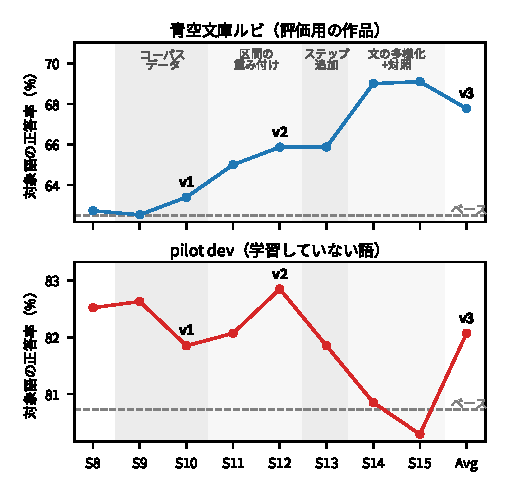
\includegraphics[width=\columnwidth]{fig_progress_ja.pdf}
\caption{段階ごとの評価セットでの正答率。青空文庫は区間の重み付けと例文の多様化で伸びる。pilot dev
（学習していない語）は長く学習するほど下がる。S12 と S15 の平均（Avg、v3 として公開）は青空文庫の
伸びの大半を残し、pilot dev を戻す。}
\label{fig:progress}
\end{figure}

\textbf{損失の希釈}（表~\ref{tab:diag}）\quad v1 の時点では、生徒は Wikipedia と青空文庫の難しい学習行を、
LLM の行よりずっと覚えられていなかった（30\%/18\% に対して 66\%）。原因を調べるため、ベースから
難しい行だけで、各行を同じ回数（24 回）学習した。Wikipedia の行は LLM の行と同じ速さで覚えられた。
差は主に、学習した回数の少なさと、長い文で対象語が薄まることから来ていた。対象語区間の重み付けが
最も効いた。8 層に増やしても効くが学習は 1.5 倍かかり、保持の損失を弱めるのは最も効かなかった。

\begin{table}[t]
\centering\footnotesize
\caption{当てはまりの診断（ベースから、各データを同じ回数学習。学習行での正答率、\%）。}
\label{tab:diag}
\begin{tabular}{@{}lrrr@{}}
\toprule
設定 & Wikipedia & 青空文庫 & LLM（M3）\\
\midrule
ベース & 12.2 & 7.6 & 8.0\\
v1 の設定 & 34.2 & 18.9 & 35.1\\
+ 区間の重み 5 & \textbf{48.2} & \textbf{28.2} & --\\
+ 上位 8 層 & 45.0 & 26.6 & --\\
+ 保持の損失 $\times0.3$ & 39.2 & 21.7 & --\\
\bottomrule
\end{tabular}
\end{table}

\textbf{丸暗記と多様化}\label{sec:variety}\quad ステップを増やすだけ（S13）でも、青空文庫の難しい学習行は
42\% から 57\% に上がった。しかし、学習した語が評価用の別の文に出てくる項目は 18\% のままだった。
生徒は語の読みではなく\emph{文}を覚えていた。語ごとの文を増やすと、これが変わった。LLM の文を 1 語
6 文足した語（S14）では、ベースが誤る評価項目の 34\% が正しく読めるようになり、以前は 20\% だった。
青空文庫の作品を 2,000 増やすと、新たに覆われた語は 8\% から 21\% になった。どの学習データにもない語は
55\% で変わらなかった。

\textbf{ずれと平均}\quad pilot dev（学習していない難しい語）は、S12 の 82.9\% から S15 の 80.3\% に下がった
（直った 11、壊れた 34、$p=8\cdot10^{-4}$）。壊れた項目の多くは、学習していない熟語の崩れた読み
だった（前庭 マエニワ$\to$ゼンニワ、活火山 $\to$ イカザン）。対照の漢字を含む普通の熟語のうち学習から
外したものは、どのモデルでも 97\% 前後を保った。したがってこれは単漢字の読みの漏れではなく、
学習していない語の緩やかなずれである。S12 と S15 を補間すると、二つの効果の釣り合いを連続的に
選べる（表~\ref{tab:interp}）。$\alpha=0.5$ を v3 とした。

\begin{table}[t]
\centering\footnotesize
\caption{S12（$\alpha{=}0$）と S15（$\alpha{=}1$）の補間。}
\label{tab:interp}
\begin{tabular}{@{}lrrrr@{}}
\toprule
$\alpha$ & 0 & 0.5 & 0.7 & 1\\
\midrule
青空文庫ルビ & 65.87 & 67.77 & 68.30 & 69.10\\
pilot dev & 82.85 & 82.07 & 81.63 & 80.29\\
Wikipedia dev & 85.09 & 84.96 & 84.99 & 85.12\\
\bottomrule
\end{tabular}
\end{table}

\begin{table}[t]
\centering
\caption{公開したチェックポイント（書き出したファイルで評価）。正答率（\%）は高いほど、CER（\%）は
低いほどよい。v3 とベースの比較（直った/壊れた）: 青空文庫 200/49（$p{=}8\cdot10^{-23}$）、Wikipedia
126/66（$p{=}2\cdot10^{-5}$）、pilot 31/20（$p{=}0.16$）、JKYB 320/96（$p{=}3\cdot10^{-29}$）。}
\label{tab:release}
\footnotesize\setlength{\tabcolsep}{3.5pt}
\begin{tabular}{@{}lrrrr@{}}
\toprule
& ベース & v1 & v2 & v3\\
\midrule
青空文庫ルビ & 62.50 & 63.30 & 65.80 & \textbf{67.53}\\
Wikipedia dev & 84.04 & 84.37 & \textbf{85.12} & 84.98\\
pilot dev & 80.73 & -- & \textbf{82.74} & 81.96\\
JSUT かな CER & 1.881 & 1.799 & 1.778 & \textbf{1.713}\\
JVS Whisper CER & \textbf{5.625} & 5.650 & 5.683 & 5.717\\
JKYB-Parakeet & 94.04 & 95.06 & 95.46 & \textbf{95.69}\\
\quad 音 / 訓 & 93.0/95.9 & 94.5/96.3 & 95.0/96.5 & 95.2/96.8\\
\bottomrule
\end{tabular}
\end{table}

\textbf{一般の文と頑健性}\quad JSUT のかな CER はどの版でも改善した（1.881\%$\to$1.713\%、改善 161 文、
悪化 99 文）。JVS の Whisper CER はばらつきの範囲で動き（改善 13、悪化 18）、その差の多くは
書き起こしの表記の揺れ（時/とき）だった。JKYB では両方の半分が改善した。初期の学習で使ってよい語は
+1.91\pt、学習から外した半分は +1.41\pt。

\textbf{シードの確認}\quad ほかの評価はすべてシード 0 で行った。青空文庫ルビをシード 1 と 2 でも測ると、
v3 はどちらでもベースより +5.73\pt 高かった（62.27\%$\to$68.00\%、直った 208・壊れた 36。
62.13\%$\to$67.87\%、209・37）。シード 0 では +5.03\pt である。

\section{議論}
\textbf{何が学ばれるか}\quad 生徒は学習した語の読みを覚え、語ごとの文脈が多様であれば、それを新しい文にも
当てはめる。一般的な読みの規則は学ばず、学習データにない語は改善しない。したがって網羅性はデータから
得るしかなく、最も安いデータは、ベースが読み誤る語について生成または検索した文である。

\textbf{限界}\quad 評価は ASR に基づき、参照音声一つで、ほとんどの評価はシード一つで行った（上のシードの確認を参照）。
kana-whisper や参照の読みが誤ることもある。試聴は非公式のものだけである。LLM の文は、読みは正しくても、
まれな語を意味の上で誤って使うことがある。BERT を共有しているため、テキストとキャプションの経路が
結び付き、絵文字のトークンはほかのトークンより大きくずれる（12--14\%）。長い継続学習は学習していない語を
ずらす。平均はこれを抑えるが、なくしはしない。

\textbf{他言語への応用}\quad この方法に必要なものは二つある。一つは、テキストエンコーダが凍結した音響モデル
から分かれている TTS モデル。もう一つは、凍結したモデルが曖昧さなく読める別の書き方で、日本語では
カタカナがその役割を果たす。文字を入力とする中国語の TTS では、多音字（行 \emph{xíng}/\emph{háng}、
长 \emph{cháng}/\emph{zhǎng} など）が同じ種類の問題になる。教師の入力では、その字を曖昧さのない同音字に
置き換えるか、モデルがピンインを読めるならピンインにすればよい。学習用の文は、多音字の辞書やコーパス
~\cite{g2pm} から作れる。ただし、これは検証していない。

\section{まとめ}
かなで読む教師に対してテキストエンコーダの上部だけを微調整すると、新しい音声なしで、凍結した
フローマッチング TTS の漢字の読みを直せる。必要な要素は四つあった。学習していない語を悪化させない
保持の損失、対象語区間の損失の重み付け、丸暗記を超えて読みを汎化させる語ごとの多様な文、ずれを
抑えるチェックポイントの平均である。公開したモデルは、一般の音声を損なわずに、評価用の文学作品の
読みを 5\pt、JKYB-Parakeet を 1.7\pt 改善した。

\section*{謝辞}
Irodori-TTS、Echo-TTS、JKYB とその Parakeet Edition、kana-whisper、JSUT・JVS コーパス、青空文庫、
Wikipedia、EDRDG の辞書ファイル、JmdictFurigana、UniDic、Sudachi、Qwen の作成者に感謝する。

\begin{thebibliography}{99}\footnotesize
\setlength{\itemsep}{0pt}
\bibitem{irodori} C.~Arata. Irodori-TTS: A flow matching-based text-to-speech model with
emoji-driven style control. Hugging Face model \texttt{Aratako/Irodori-TTS-v4.1-Small} and
\url{https://github.com/Aratako/Irodori-TTS}, 2026.
\bibitem{echo} J.~Darefsky. Echo-TTS. Blog post,
\url{https://jordandarefsky.com/blog/2025/echo/}, 2025.
\bibitem{rf} X.~Liu, C.~Gong, Q.~Liu. Flow straight and fast: Learning to generate and transfer
data with rectified flow. \emph{ICLR}, 2023.
\bibitem{fm} Y.~Lipman, R.~T.~Q.~Chen, H.~Ben-Hamu, M.~Nickel, M.~Le. Flow matching for
generative modeling. \emph{ICLR}, 2023.
\bibitem{cfg} J.~Ho, T.~Salimans. Classifier-free diffusion guidance. arXiv:2207.12598, 2022.
\bibitem{dacvae} Meta AI. DACVAE. \url{https://github.com/facebookresearch/dacvae}.
\bibitem{dac} R.~Kumar, P.~Seetharaman, A.~Luebs, I.~Kumar, K.~Kumar. High-fidelity audio
compression with improved RVQGAN. \emph{NeurIPS}, 2023.
\bibitem{modernbert} B.~Warner et al. Smarter, better, faster, longer: A modern bidirectional
encoder for fast, memory efficient, and long context finetuning and inference.
arXiv:2412.13663, 2024.
\bibitem{modernbertja} SB Intuitions. \texttt{sbintuitions/modernbert-ja-310m}. Hugging Face,
2025.
\bibitem{jkyb} SB Intuitions. Joyo Kanji Yomi Benchmark.
\url{https://github.com/sbintuitions/Joyo-Kanji-Yomi-Benchmark}.
\bibitem{jkybp} Parakeet Inc. Joyo Kanji Yomi Benchmark, Parakeet Edition (JKYB-Parakeet).
\url{https://github.com/Parakeet-Inc/Joyo-Kanji-Yomi-Benchmark-Parakeet-Edition}.
\bibitem{kanawhisper} SB Intuitions. \texttt{sbintuitions/kana-whisper}. Hugging Face.
\bibitem{whisper} A.~Radford et al. Robust speech recognition via large-scale weak supervision.
\emph{ICML}, 2023.
\bibitem{jsut} R.~Sonobe, S.~Takamichi, H.~Saruwatari. JSUT corpus: free large-scale Japanese
speech corpus for end-to-end speech synthesis. arXiv:1711.00354, 2017.
\bibitem{jvs} S.~Takamichi et al. JVS corpus: free Japanese multi-speaker voice corpus.
arXiv:1908.06248, 2019.
\bibitem{mcnemar} Q.~McNemar. Note on the sampling error of the difference between correlated
proportions or percentages. \emph{Psychometrika}, 12(2):153--157, 1947.
\bibitem{mecab} T.~Kudo, K.~Yamamoto, Y.~Matsumoto. Applying conditional random fields to
Japanese morphological analysis. \emph{EMNLP}, 2004.
\bibitem{unidic} Y.~Den, J.~Nakamura, T.~Ogiso, H.~Ogura. A proper approach to Japanese
morphological analysis: Dictionary, model, and evaluation. \emph{LREC}, 2008.
\bibitem{sudachi} K.~Takaoka et al. Sudachi: a Japanese tokenizer for business. \emph{LREC}, 2018.
\bibitem{jmdict} J.~Breen. JMdict: a Japanese-multilingual dictionary. \emph{COLING Workshop on
Multilingual Linguistic Resources}, 2004.
\bibitem{jmdictfurigana} Doublevil. JmdictFurigana.
\url{https://github.com/Doublevil/JmdictFurigana}.
\bibitem{qwen3} Qwen Team. Qwen3 technical report. arXiv:2505.09388, 2025.
\bibitem{vllm} W.~Kwon et al. Efficient memory management for large language model serving with
PagedAttention. \emph{SOSP}, 2023.
\bibitem{wiseft} M.~Wortsman et al. Robust fine-tuning of zero-shot models. \emph{CVPR}, 2022.
\bibitem{soups} M.~Wortsman et al. Model soups: averaging weights of multiple fine-tuned models
improves accuracy without increasing inference time. \emph{ICML}, 2022.
\bibitem{g2pm} K.~Park, S.~Lee. g2pM: A neural grapheme-to-phoneme conversion package for
Mandarin Chinese based on a new open benchmark dataset. \emph{Interspeech}, 2020.
\end{thebibliography}
\end{document}
